\documentclass[a4paper, 11pt]{article}
\usepackage{comment} % enables the use of multi-line comments (\ifx \fi) 

\usepackage{fullpage} % changes the margin
\usepackage{longtable}
\usepackage{graphicx}
\usepackage{fancyvrb,xcolor}
\usepackage{listings}
\usepackage{color}
\usepackage[margin=3cm]{geometry}
\usepackage{relsize}
\definecolor{dkgreen}{rgb}{0,0.6,0}
\definecolor{gray}{rgb}{0.5,0.5,0.5}
\definecolor{mauve}{rgb}{0.58,0,0.82}
\definecolor{LightCyan}{rgb}{0.88,1,1}
\usepackage{float}
\usepackage{caption}
\DeclareCaptionFont{white}{\color{white}}
\DeclareCaptionFormat{listing}{\colorbox{gray}{\parbox{\textwidth}{#1#2#3}}}
\captionsetup[lstlisting]{format=listing,labelfont=white,textfont=white}
\newcommand{\bigqm}[1][1]{\text{\larger[#1]{\textbf{?}}}}
\lstset{
  language=Java,
  aboveskip=3mm,
  belowskip=3mm,
  showstringspaces=false,
  columns=flexible,
  basicstyle={\small\ttfamily},
  numbers=none,
  numberstyle=\tiny\color{gray},
  keywordstyle=\color{blue},
  commentstyle=\color{dkgreen},
  stringstyle=\color{mauve},
  breaklines=true,
  breakatwhitespace=true,
  tabsize=3
}
\graphicspath{ {images/} }

\begin{document}
%Header-Make sure you update this information!!!!
\noindent
\large\textbf{Assignment 3} \hfill \textbf{Hussam Hallak} \\
\normalsize CS834, Information Retrieval, Fall 2017\hfill CS Master's Student \\
Old Dominion University, Computer Science Dept \hfill Prof: Dr. Nelson 

\section*{Question 1:}
Exercise 6.1: 

Using the Wikipedia collection provided at the book website, create a sample of stem clusters by the following process:

1. Index the collection without stemming.

2. Identify the first 1,000 words (in alphabetical order) in the index.

3. Create stem classes by stemming these 1,000 words and recording which words become the same stem.

4. Compute association measures (Dice’s coefficient) between all pairs of stems in each stem class. Compute co-occurrence at the document level.

5. Create stem clusters by thresholding the association measure. All terms that are still connected to each other form the clusters.

Compare the stem clusters to the stem classes in terms of size and the quality (in
your opinion) of the groupings.



\subsection*{Answer:}
First, I modified the code I wrote for Assignment \#2 Question \#4 to build the inverted index. The program is written in python, and the source code file is named ``inverted.py''. I have used the WikiSmall collection provided on the book website as a sample:

http://www.search-engines-book.com/collections/

The program extracts all html documents and stores the unique words in each document as a key-value pair where
the document is the key and the words are the value. Swapping the key and the value will generate the inverted index we need. The output is printed on the screen and saved to the file ``inverted.txt''.


I have chosen Google and Bing search engines. The technique described in this chapter uses the formula:

$$
N=\frac{f_a \times f_b}{f_{ab}}
$$

Where:

$a$ and $b$ are the independent terms

$N$ is the estimated total number of indexed pages

$f_a$ is the number of pages containing the term $a$

$f_b$ is the number of pages containing the term $b$

$f_{ab}$ is the number of pages containing both $a$ and $b$

\paragraph{•}
The two terms in the query need to be as independent as possible, so I have chosen the following queries:

1. Diesel Memory

2. Hairy Phone

3. Computer Manifold

4. Electronic Lumber

\paragraph{1. Diesel Memory:}
I ran the first query ``Diesel Memory'' and found the following:

A. Google:

\pagebreak
Google found about 207,000,000 results for the term ``Diesel''.
\begin{figure}[h]
\caption{Query: Diesel, Search Engine: Google}
\centering
%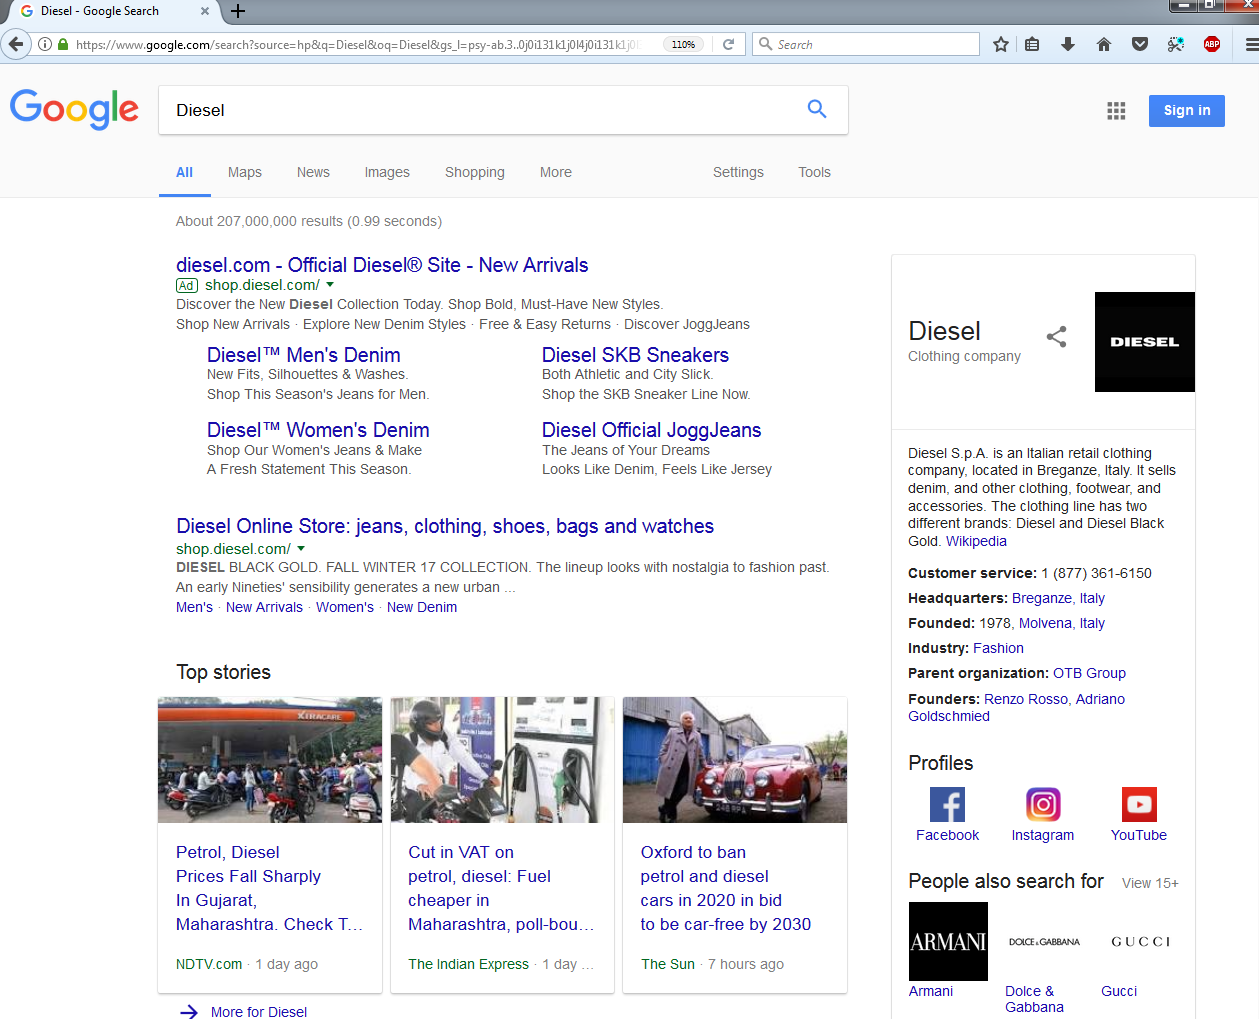
\includegraphics[scale=0.4]{Q1/DieselGoogle.png}
\end{figure}

\pagebreak
Google found about 377,000,000 results for the term ``Memory''.
\begin{figure}[h]
\caption{Query: Memory, Search Engine: Google}
\centering
%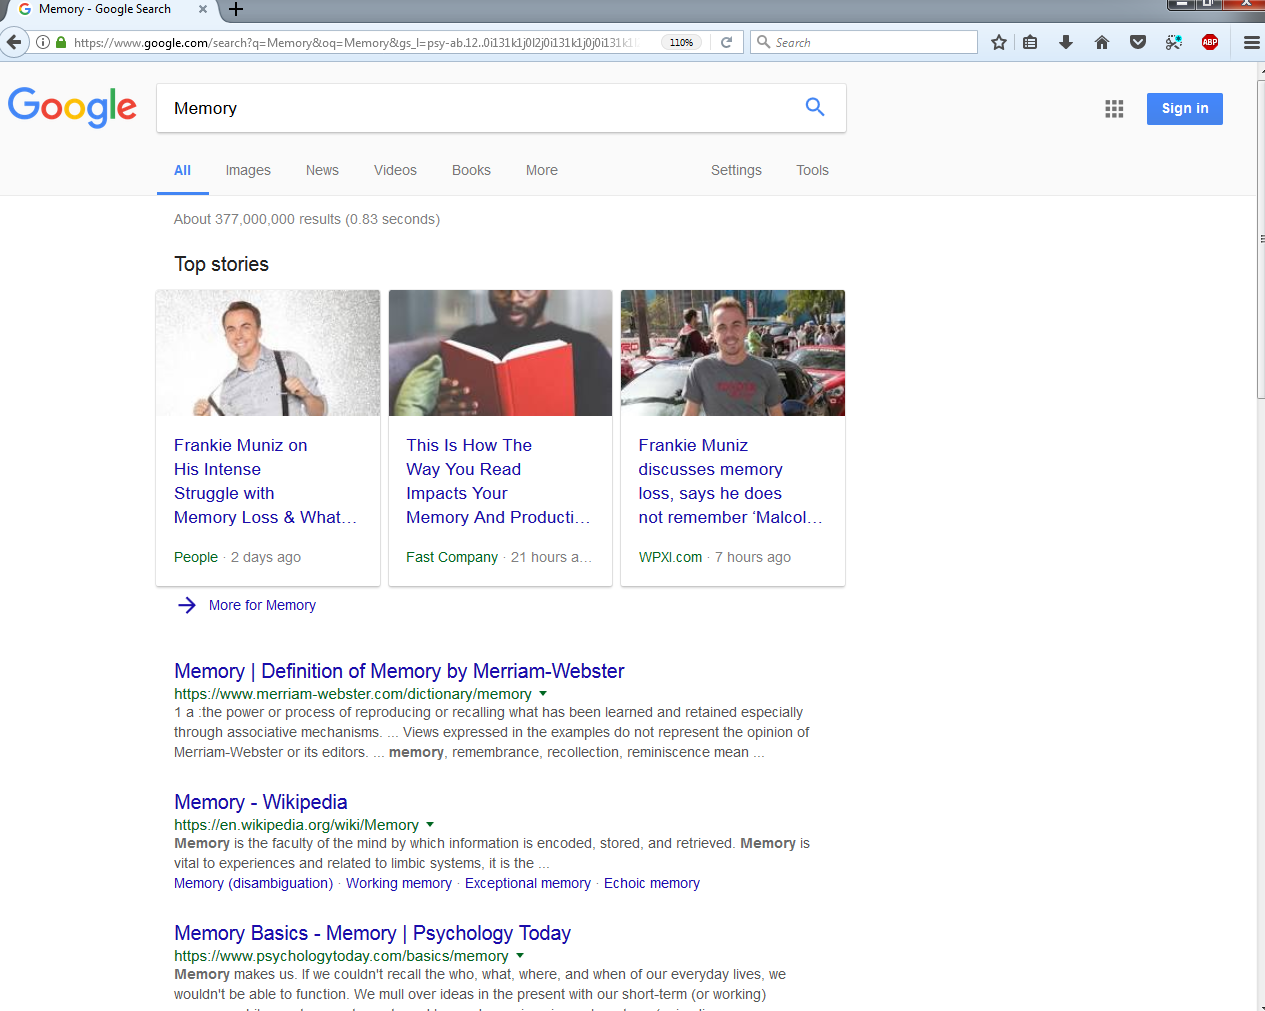
\includegraphics[scale=0.4]{Q1/MemoryGoogle.png}
\end{figure}

\pagebreak
Google found about 36,900,000 results for the query ``Diesel Memory''.
\begin{figure}[h]
\caption{Query: Diesel Memory, Search Engine: Google}
\centering
%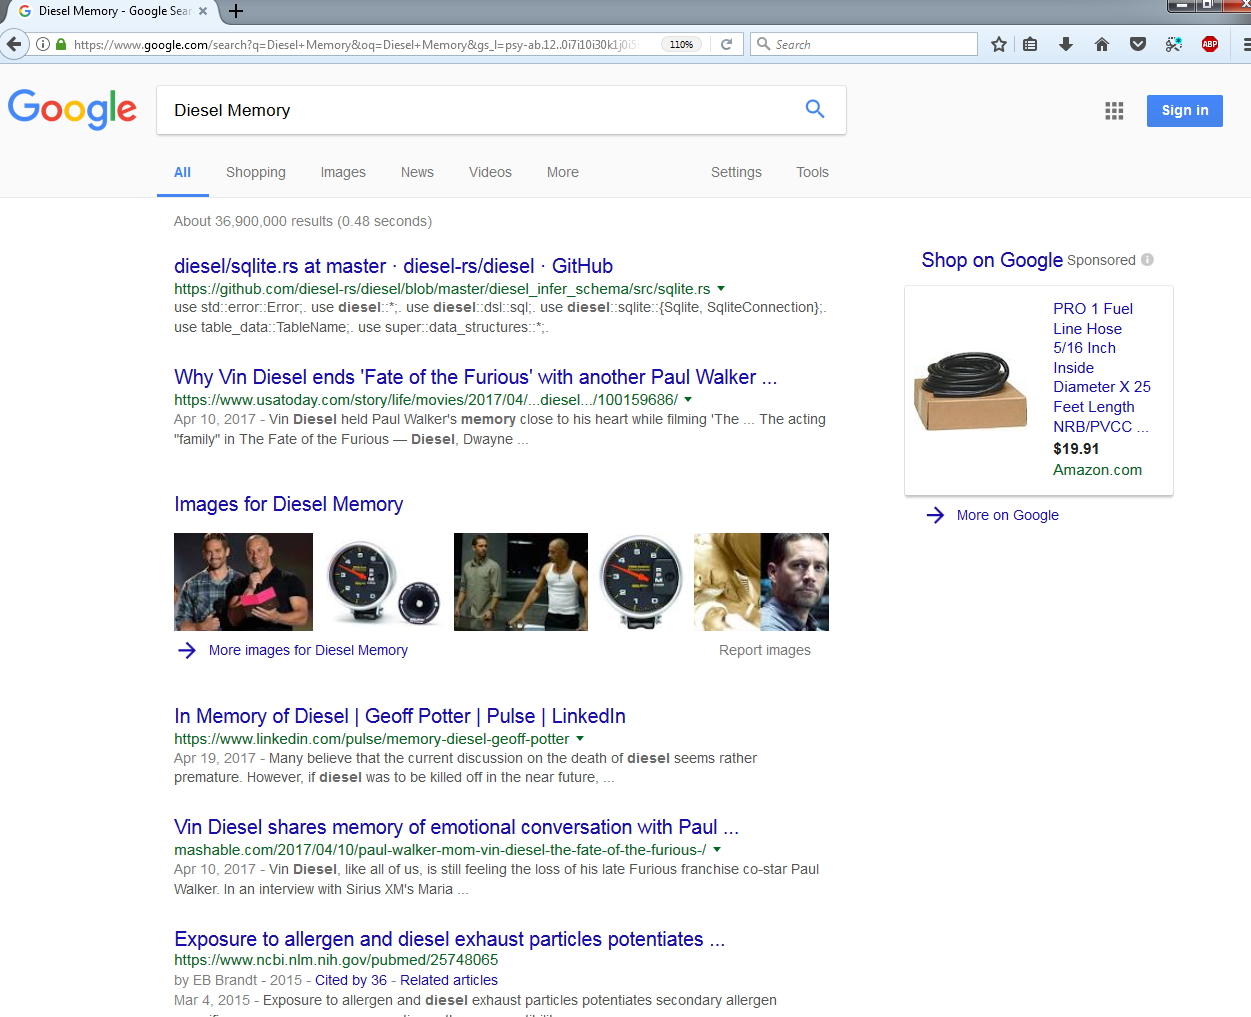
\includegraphics[scale=0.4]{Q1/DieselMemoryGoogle.png}
\end{figure}

Plugging the results in the formula gives the following:

$$N_{google} = \frac{207,000,000 \times 377,000,000}{36,900,000} = 2114878048.780488 \approx 2114878049
$$


\pagebreak

B. Bing:

Bing found about 183,000,000 results for the term ``Diesel''.

Plugging the results in the formula gives the following:

$$N_{Bing} = \frac{183,000,000 \times 167,000,000}{3,220,000} = 9490993788.819876 \approx 9490993789
$$


\paragraph{2. Hairy Phone:}
I ran the second query ``Hairy Phone'' and found the following:

A. Google:

Google found about 106,000,000 results for the term ``Hairy''.

Google found about 1,410,000,000 results for the term ``Phone''.

Google found about 8,780,000 results for the query ``Hairy Phone''.

Plugging the results in the formula gives the following:

$$N_{google} = \frac{106,000,000 \times 1,410,000,000}{8,780,000} = 17022779043.28018 \approx 17022779043
$$

B. Bing:

Bing found about 292,000,000 results for the term ``Hairy''.

Bing found about 748,000,000 results for the term ``Phone''.

Bing found about 51,500,000 results for the query ``Hairy Phone''.

Plugging the results in the formula gives the following:

$$N_{Bing} = \frac{292,000,000 \times 748,000,000}{51,500,000} = 4241087378.640777 \approx 4241087379
$$

\paragraph{3. Computer Manifold:}
I ran the third query ``Computer Manifold'' and found the following:

A. Google:

Google found about 861,000,000 results for the term ``Computer''.

Google found about 21,500,000 results for the term ``Manifold''.

Google found about 6,470,000 results for the query ``Computer Manifold''.

Plugging the results in the formula gives the following:

$$N_{google} = \frac{861,000,000 \times 21,500,000}{6,470,000} = 2861128284.38949 \approx 2861128284
$$

B. Bing:

Bing found about 448,000,000 results for the term ``Computer''.

Bing found about 38,400,000 results for the term ``Manifold''.

Bing found about 35,100,000 results for the query ``Computer Manifold''.

Plugging the results in the formula gives the following:

$$N_{Bing} = \frac{448,000,000 \times 38,400,000}{35,100,000} = 490119658.1196581 \approx 490119658
$$

\paragraph{4. Electronic Lumber:}
I ran the forth query ``Electronic Lumber'' and found the following:

A. Google:

Google found about 1,010,000,000 results for the term ``Electronic''.

Google found about 43,300,000 results for the term ``Lumber''.

Google found about 5,720,000 results for the query ``Electronic Lumber''.

Plugging the results in the formula gives the following:

$$N_{google} = \frac{1,010,000,000 \times 43,300,000}{5,720,000} = 7645629370.629371 \approx 7645629371
$$

B. Bing:

Bing found about 289,000,000 results for the term ``Electronic''.

Bing found about 42,400,000 results for the term ``Lumber''.

Bing found about 244,000,000 results for the query ``Electronic Lumber''.

Plugging the results in the formula gives the following:

$$N_{Bing} = \frac{289,000,000 \times 42,400,000}{244,000,000} = 50219672.13114754 \approx 50219672
$$

The estimated number of indexed pages in Google as I found are:

2114878049

17022779043

2861128284

7645629371

It is clear that the estimates varied markedly, by few billions, for different queries. I assume that one of the reasons behind that is the difference in ``independence level'' of the two terms among different queries.

The estimated number of indexed pages in Bing as I found are:

9490993789

4241087379

490119658

50219672

The same inconsistency held for Bing. The estimates varied by few billions.


\section*{Question 2:}
Exercise 4.6:

Create a simple spelling corrector based on the noisy channel model. Use a single-word language model, and an error model where all errors with the same edit distance have the same probability. Only consider edit distances of 1 or 2. Implement your own edit distance calculator (example code can easily be found on the Web).

\section*{Answer:}

I wrote a simple python script ``PKstem.py'' to process the documents, stem the unique words in them, using Porter and Krovetz stemmers. The stemmers were not implemented from scratch because there are python libraries for both stemmers already.

%\lstinputlisting[language=Python, breakatwhitespace=〈false), label=The content of PKstem.py, caption= The content of PKstem.py]{Q2/PKstem.py}

The program accepts the document(s) file name(s) as command line argument(s). It is possible to run the program and process all files at once, however, I ran each file separately.

After running the documents, I found the following results:

\textbf{Aakrosh\_(1998\_film).html}

Unique words: 229

Porter stems: 224

Krovetz stems: 227
 
\textbf{Aargau\_frank.html}

Unique words: 199

Porter stems: 193

Krovetz stems: 193

\textbf{Aaron\_Chalmers\_3ab5.html}

Unique words: 154

Porter stems: 149

Krovetz stems: 150

\textbf{Baba\_Budan\_67b5.html}

Unique words: 92

Porter stems: 90

Krovetz stems: 91

\textbf{Babs\_Fafunwa\_5f48.html}

Unique words: 239

Porter stems: 231

Krovetz stems: 235

This is a screen shot of running the program on the first file:




I found the following examples of differences in the stemming that could have an impact on ranking:

\begin{longtable}{ |p{3cm}|p{3cm}|p{3cm}| } 
\hline
Word & Porter Stem & Krovetz Stem \\
 \hline 
 daily & daili & daily \\
 \hline
  changes & chang & change \\
 \hline
  academic & academ & academic \\
 \hline
  collaboration & collabor & collaboration \\
 \hline
  manchester & manchest & manchester \\
 \hline
  denominations & denomin & denomination \\
 \hline
  circulating & circul & circulate \\
 \hline
  article & articl & article \\
 \hline
  versus & versu & versus \\
 \hline
  association & associ & association \\
 \hline
\end{longtable}



\section*{Question 3:}
Exercise 4.8:

Find the 10 Wikipedia documents with the most inlinks. Show the collection of anchor text for those pages.

\section*{Answer:}

In order to find the 10 Wikipedia documents with the most inlinks, I created a small python script ``inlinks.py'' that extracts all links found in Wikipedia documents from WikiSmall collection. I stored the links as a key-value pair, where file name is the key and the link is the value. After grouping the links by their ``href'' value, I counted them and sorted the files by the number of inlinks to find the top 10  Wikipedia documents with the most inlinks.


The program writes the result to a file ``output.txt''. This is a screen shot of the file:



\section*{Question 4:}
Exercise 6.4: 

Assuming you had a gazetteer of place names available, sketch out an algorithm for detecting place names or locations in queries. Show examples of the types of queries where your algorithm would succeed and where it would fail.

\subsection*{Answer:}
The easiest way to detect place names or locations in a query is to tokenize the query and run all tokens against the place names dictionary, gazetteer. This method would be computationally expensive if the gazetteer has a large number of place names. It will sometimes fail, generate some false positives. For example:

Query: Virginia Woolf

The term ``Virginia'' will be falsely identified as a place name, but the user meant Virginia Woolf, the writer.

A better, less expensive, algorithm can be implemented by defining patterns that will help detecting place names. These patterns can be defined using prepositions or other words that are used with places in English language. Examples of these prepositions and words include: From, in, near, to, of, ...etc.

Pattern: $* + ('in' || 'from' || 'near' || 'to' || 'of' ) + <place name>$

Example queries:

Celebrities born in Virginia

When did MalcomX go to Egypt

Universities in Hampton

Homes for sale near Suffolk  

Is Michael Nelson from Norfolk

Does Syria lie north of Jordan?

The approach would begin by scanning the query to find these words or prepositions from, in, to, ...etc. If one of the words is detected, only the following word is run through the gazetteer. This method will sometimes fail, generate some false positives as well as false negatives. 

False positive example:

Query: A recipe for a pie made out of avocado

The term ``avocado'' will be falsely detected as a place name, Avocado, California. However, the user meant avocado, the fruit.

False negative example:

Query: Where is Avocado located in California?

Unless the defined patterns are advanced enough to detect place names in such queries, ``Avocado'', the place in California will not be detected.

Assuming that the defined patterns are advanced enough to identify all possible place names, practically impossible, a large amount of False positives will be generated.

Pattern: $<place name> + location$

Query 1: Washington location on the map

Query 2: George Washington location of birth

In query 1, the term ``Washington'' will be detected as a place name, which is true. However, the same term ``Washington'' in query 2 will also be identified as a place name, which is false.

Also using patterns will have to be accompanied with a rule to handle single term queries. This will also generate a large number of false positives. For example:

Query: Lincoln

The term ``Lincoln'' will be identified as the place name Lincoln in Alabama, while the user's intention was to look up Lincoln, the president or Lincoln, the car or Lincoln, the welding machine.

One more rule must be added to the patterns to handle place names that are not a single terms. Examples include place names like ``Virginia Beach'', ``Newport News'', ``Washington DC'', ...etc.

Example:

Pattern: $* + ('in' || 'from' || 'near' || 'to' || 'of' ) + <place name>$

Query: Hospitals in San Francisco

A rule to handle queries similar to the query above must be added. The first word of each place name that is n-gram where $n > 1$ must be added to the gazetteer and then mapped to the next term in the place name.

Here is my simple algorithm/implementation to detect place names in python-like code:


Success example:

Query: Schools in Norfolk

Failure example:

Query: Casinos in Las Vegas

\section*{Question 5:}
Exercise 7.5: 

Implement a BM25 module for Galago. Show that it works and document
it.

\subsection*{Answer:}

I wrote the code for BM25 in Java since that is the language in which Galago is written. The file is named ``BM25.java''. Some variables should be passed as arguments, but for the purpose of demonstration, I manually set them within the class BM25. Here is the code I wrote:



I downloaded the source code for Galago. BM25 is already implemented in the file ``BM25Scorer.java''. I noticed that IDF is calculated using a different formula. Here is the formula used in their implementation:

\begin{lstlisting}
idf = Math.log(documentCount / (df + 0.5)); 
\end{lstlisting}




\begin{thebibliography}{9}

\bibitem{} 
Stackoverflow. https://stackoverflow.com/questions/tagged/python.

\bibitem{} 
https://stackoverflow.com/questions/10369393/need-a-python-module-for-stemming-of-text-documents

\bibitem{}
https://www.rosettacode.org/wiki/Inverted\_index\#Simple\_inverted\_index

\bibitem{}
https://en.wikipedia.org/wiki/Pigeonhole\_principle


\end{thebibliography}


\end{document}